\section{Related Work}
\label{related}

\begin{figure*}[t]
\centering
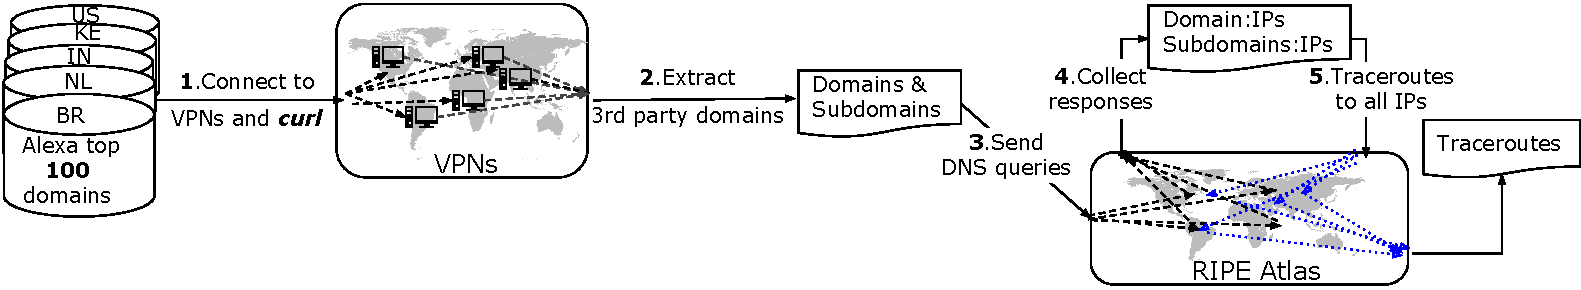
\includegraphics[width=.9\textwidth]{Current-Traffic_fig}
\caption{Measurement pipeline to study Internet paths from countries to
  popular domains.}
\label{fig:pipeline1}
\end{figure*}

{\bf Nation-state routing analysis.}  Shah and
Papadopoulos recently measured international routing detours---paths that originate
in
one country, cross international borders, and then return to the
original country---using public Border Gateway Protocol~(BGP) routing tables~\cite
{shah2015characterizing}. 
The study discovered 2~million detours each month out
of 7 billion paths.
%JEN: hard to understand.  doesn't seem important.
%the study also characterized the detours based
%on detour dynamics and persistence.  
Our work differs by {\em actively}
measuring Internet paths using traceroute, yielding a more precise (and accurate) measurement of the paths, %traffic is
%likely to take
as opposed to analyzing BGP
routes.  Obar and Clement analyzed traceroutes
that started and ended in Canada, but tromboned through the United
States, and argued that
this is a violation of Canadian network
sovereignty~\cite{obar2012internet}. 
Karlin \ea{} developed a framework for country-level
routing analysis to study how much influence each country has over
interdomain routing~\cite{karlin2009nation}.  This work measures country
centrality using BGP routes and AS-path inference; in contrast, our work uses active 
measurements and measures avoidability of a given country. 

{\bf Mapping national Internet topologies.}  Roberts \ea{} developed a method
for mapping national networks and identifying ASes that act as points of
control~\cite{roberts2011mapping}.   %JEN: not clear we care about the
 Several studies have also characterized network paths {\em
within} a country, including
Germany~\cite{wahlisch2010framework,wahlisch2012exposing} and
China~\cite{zhou2007chinese}, or a country's interconnectivity %within a region
%or with the rest of theworld~
\cite{bischof2015and,gupta2014peering,fanou2015diversity}; these studies
focus on paths within a country, as opposed to paths that traverse multiple countries.

{\bf Routing overlays and Internet architectures.} Alibi Routing uses
round-trip times to prove that that a client's packets did  not traverse a
forbidden country or region~\cite{levin2015alibi,levin_detour}; \system{} differs by
measuring  which countries a client's packets traverse.  Our
work then  uses active measurements to determine the best path for a client
wishing  to connect to a server.  RON, Resilient Overlay Network, is an
overlay network that  routes around failures~\cite{andersen2001resilient}, whereas our overlay network
routes around countries.  ARROW introduces a
model that allows users to route around ISPs~\cite{peter2015one}, but requires
ISP participation, making it considerably more difficult to deploy than
\system{}. ARROW also aims to improve fault-tolerance, robustness, and
security, rather than explicitly attempting to avoid certain countries; ARROW
provides mechanisms to avoid individual ISPs, but such a mechanism is at a
different level of granularity, because an ISP may span multiple countries.
Zhang \ea{} presented SCION, a ``clean-slate'' Internet architecture that
provides route control, failure isolation, and explicit trust information for
communication~\cite{zhang2011scion}; SCION, however, requires fundamental
changes to the Internet architecture, whereas \system{} is deployable today.

{\bf Circumvention systems.}  Certain tools, such as anonymous
communications systems or VPNs~\cite{dingledine2004tor,nobori2014vpn,piotrowska2017loopix,van2015vuvuzela,wolinsky2012dissent,tyagi2016stadium,corrigan2015riposte,kwon2016atom,kwon2016riffle,
gelernter2016two}, use a combination of
encryption and overlay routing to allow clients to avoid censorship and surveillance. Tor is
an anonymity system that uses three relays and layered encryption to allow
users to communicate anonymously~\cite{dingledine2004tor}.  In contrast,
\system{} does not aim to achieve anonymity; instead, its aim is to ensure
that traffic does not traverse a specific  country, a goal that Tor cannot
achieve.  Even tools like Tor do not inherently thwart surveillance: Tor is
vulnerable to traffic correlation attacks and some attacks are possible even
on encrypted user traffic. VPNGate is a public VPN relay system aimed at
circumventing national firewalls~\cite{nobori2014vpn}. Unfortunately, VPNGate
does not allow a client to choose any available VPN endpoint, which makes it more
difficult for a user to ensure that traffic avoids a particular country.  
Neither of these systems explicitly avoid or route around countries. Additionally, existing circumvention systems generally rely on
encryption, which is different from \system{}; prior research has shown that
websites can be fingerprinted based on size, content, and location of third
party resources, which  reveals information about the content a user is
accessing \cite{what_isps_can_see}.  Finally, ISPs often execute man-in-the-middle attacks on TLS connections to perform network-management
functions~\cite{mitm_isp}.

